\chapter{Night 1: Introduction to Matrices}

\section*{Overview and Orientation}
In this night assignment, we will learn some of the foundational material about matrices and matrix operations.

\begin{learningobjectives}
\emph{Concepts}
\bi
\item Define a vector, a matrix and an array
\item Describe the meaning of the dimensions of a vector, a matrix, and an array
\item Give at least one interpretation of matrix-vector multiplication
\item Calculate the product of a matrix-vector multiplication for 2D and 3D matrices
\item Understand dimensionality-requirements for matrix-vector multiplication and predict resulting dimensions
\item Define and recognize the following special matrices: Identity, diagonal, square, rectangular, symmetric
\ei
\emph{MATLAB skills}
\bi
\item Determine the dimensions of a vector, matrix, or array variable
\item Perform operations (addition, multiplication, transposition) on matrices
\item Extract desired subarrays or matrices from arrays
\ei
\end{learningobjectives}

\subsection{Suggested Approach}

\begin{itemize}
\item First you should quickly scan through the assignment, see what is
being asked, and assess the extent to which you already know how
to do things. Spend no more than 30 minutes or so doing this.

\item You should then read the assignment more closely, try out problems, and if appropriate, look at some of the other resources that are suggested. Don't spend more than 1 hour poking around at stuff online unless it is really being productive: it's easy to spend a lot of time there without accomplishing much.

\item Then start doing the problems in earnest, and/or spend focused time with suggested resources.

\item Once you've spent a total of 3-4 hours working on the assignment, you should check your progress. Are you on track to finish within about 7-8 hours? Do you feel confident that you can do the stuff that's left? If not, this is when you should ask for help. This means talk to a colleague, or talk to a ninja, or track down an instructor, or send an email to an instructor.

\item You should turn in a PDF document with answers to all the numbered questions below. For the MATLAB assignments, please export your work to pdf. Please carefully label the problem number in your MATLAB script.

\end{itemize}

\subsection{Resources to read and watch}

There are lots of books about Linear Algebra and lots of useful videos on the web. Here are some specific recommendations:
\begin{itemize}
\item Introduction to Linear Algebra, by Strang
\item Linear Algebra, by Lay
\item \href{https://www.math.ucdavis.edu/~linear/}{Linear Algebra, by Cherney, Denton, Thomas, Waldron}
\item Homebrew videos
\begin{itemize}
\item \href{https://youtu.be/XSNHG1Vkcik}{Matrices operating on vectors}
\item \href{https://youtu.be/T5Larkrb430}{Matrices operating on vectors (example)}
\item \href{https://youtu.be/_cQq85Th6nI}{Matrices operating on matrices}
\end{itemize}
\item Videos from others
\begin{itemize}
\item \href{https://youtu.be/fNk_zzaMoSs}{Vectors, the very basics}
\item \href{https://www.youtube.com/playlist?list=PLZHQObOWTQDPD3MizzM2xVFitgF8hE_ab}{3Blue1Brown's YouTube series on Linear Algebra}
\end{itemize}
\end{itemize}

%Add in references to squeeze, reshape, other useful Matlab commands!!!  2_26_18
%Fix sign conventions in rotation matrices 2_26_18
%Give more info on how they are supposed to assign temps to cities (north-south)  2_26_18


\section{Linear Algebra, Vectors, and Matrices}

In your concept-maps for eigenfaces, most, if not all of you would have included something about linear algebra, matrices, and vectors. These topics are used very heavily in many different areas, including in data analysis. For the next couple of weeks, you will spend a good deal of time learning about these things and how to apply them.

\subsection{Linear Algebra and Vectors}

\begin{center}
\begin{tikzpicture}[scale=.3]
\draw [<->,gray!50!black] (0,5) node[above]{$z$} -- (0,0) --(-3,-4) node[left]{$x$};
\draw [->,gray!50!black] (0,0)--(5,0) node[right]{$y$};

\draw [->,red] (0,0)--(7,-9) node[midway,above] {$\mathbf{v}$};

\node[right] at (7,-9) {$p$};

\end{tikzpicture}
\end{center}

Consider the point $p = (1,2,-1)$ in 3-dimensional space. We can associate a position vector $\mathbf{v}$ with this point, which is the vector from the origin to this point,
\[\mathbf{v} = \left[
\begin{array}{r}
1 \\
2 \\
-1
\end{array}\right].
\]
Likewise, we can think of every vector as defining a point, if we assume that the vector emanates from the origin. So, for example, the vector
\[\mathbf{v} = \left[
\begin{array}{r}
3 \\
-2 \\
0 \\
1
\end{array}\right]
\]
is identified with the point $(3,-2,0,1)$ in 4D. Often times we will mix and match these ideas and say things like: the vector $(x,y,z)$. What we really mean when we say this is: the point $(x,y,z)$ can be treated as the position vector
\[\mathbf{v} = \left[
\begin{array}{r}
x \\
y \\
z
\end{array}\right]
\]

The vector $\mathbf{v}$, as represented above, is called a column vector. We can also have row vectors such as the following
 \begin{align*}
 \mathbf{u} = \begin{bmatrix} p & q & r \end{bmatrix}.
 \end{align*}

The operation of converting a column vector to a row vector or vice-versa is called taking the \emph{transpose} of the vector and is denoted with a superscript $T$. For example, the transpose of the row vector $\mathbf{u}$ from above is
\begin{align}
\mathbf{u}^T &= \begin{bmatrix} p \\ q \\ r \end{bmatrix}
\end{align}
and the transpose of the vector $\mathbf{v}$ from above is 
\begin{align}
\mathbf{v}^T &= \begin{bmatrix} x & y & z \end{bmatrix}.
\end{align}

We can take the product of a row vector with a column vector using the following formula
\begin{align}
\mathbf{u}\mathbf{v} =  \begin{bmatrix} p & q & r \end{bmatrix}\begin{bmatrix}
x \\
y \\
z
\end{bmatrix}  = px + qy + zr
\end{align}

If we start with two column vectors $$\mathbf{v} = \begin{bmatrix} v_1 \\ v_2 \\ \vdots \\ v_n \end{bmatrix} \text{ and } \mathbf{w}=\begin{bmatrix}
w_1 \\ w_2 \\ \vdots \\ w_n
\end{bmatrix}$$ of length $n$ (i.e., they are $n$=dimensional), then we can take the {\textit dot product}
$$\mathbf{v}\cdot \mathbf{w} = v_1w_1 + v_2w_2 + \cdots + v_nw_n.$$
In some sense, the dot product is a measure of how aligned two vectors are. Here's the key formula:
$$\mathbf{v}\cdot\mathbf{w} = \|\mathbf{v}\|\|\mathbf{w}\|\cos\theta$$
where $\theta$ is the angle between $\mathbf{v}$ and $\mathbf{w}$ and 
$$\|\mathbf{v}\|=\sqrt{v_1^2 + v_2^2 + \cdots + v_n^2}^{1/2}$$
is the length of the vector $\mathbf{v}$ in $n$-dimensional space.
\begin{prob}
\begin{enumerate}
    \item Assume $\mathbf{v}$ and $\mathbf{w}$ are two vectors of unit length, i.e., $\|\mathbf{v}\| = \|\mathbf{w}\|=1$. Using the formula above, what angle between $\mathbf{v}$ and $\mathbf{w}$ maximizes the dot product? Using the formula above, what angle between $\mathbf{v}$ and $\mathbf{w}$ minimizes the dot product?
    \item Compute $\mathbf{v}\cdot\mathbf{w}$ where
    $$\mathbf{v} = \begin{bmatrix}
    1 \\ 3 \\ -4 \\ 6
    \end{bmatrix}, \text{ and } \mathbf{w}=\begin{bmatrix}
    -2 \\ 0 \\ 1 \\ 3
    \end{bmatrix}$$
    \end{enumerate}
\end{prob}
\begin{sol}
\begin{enumerate}
    \item 
Using the formula, $\mathbf{v}\cdot\mathbf{w}=\cos(\theta)$. So, when $\theta=0$, (i.e., the vectors point in the same direction) the dot product is maximized and when $\theta=\pi/2$ (i.e., the vectors are perpendicular) the dot product is minimized.
\item The dot product is
$$\mathbf{v}\cdot\mathbf{w} = -2 + 0 -4 + 18 = 12$$
\end{enumerate}
\end{sol}
We'll learn more about the dot product as we go. For now, notice that the dot product equals the product of the transpose of one with the other
\begin{align}
\mathbf{v}\cdot \mathbf{w} = \mathbf{v}^T \mathbf{w}.
\end{align}

Vectors can also be used to represent many things, such as data. Linear algebra provides a powerful set of tools to manipulate and analyze this data.

\begin{prob}
\label{ex:fruit}
For instance, you may have a three-dimensional vector $\mathbf{f}$ whose entries represent the numbers of different fruits you have in your refrigerator. For example, the first entry could be the number of oranges, the second the number of grapefruits and the third could be the number of apples. When organized in this manner, you can use products of row and column vectors to compute the number of different fruits there are. For instance, suppose that

\begin{align}
\mathbf{f} = \begin{bmatrix}
1 \\ 2 \\ 3
\end{bmatrix},
\end{align}
 i.e. you have 1 orange, 2 grapefruits, and 3 apples in your fridge.

\begin{enumerate}
\item Find a row vector $\mathbf{t}$ so that the product $\mathbf{t} \mathbf{f}$ tells you the total number of fruits in your refrigerator.
\item Find a row vector $\mathbf{c}$ such that the product $\mathbf{c}\mathbf{f}$ tells you the total number of \emph{citrus} fruits in your refrigerator.
\item Suppose that in the genetically engineered future, all apples weigh 100 g, all grapefruits weigh 250 g and all oranges weigh 120 g. Find a row vector $\mathbf{w}$, such that the product $\mathbf{w}\mathbf{f}$ tells you the total weight of fruits in your refrigerator.
\end{enumerate}
\end{prob}

\begin{sol}
\begin{enumerate}
    \item Let $\mathbf{t} = \begin{bmatrix}
        1 & 1 & 1
    \end{bmatrix}$. Then $\mathbf{t}\mathbf{f} = 1 + 2 + 3 = 6$, the total number of fruits in your refrigerator.
    \item Let $\mathbf{c} = \begin{bmatrix}
        1 & 1 & 0
    \end{bmatrix}$. Then $\mathbf{c}\mathbf{f} = 1 + 2 + 0 = 3$, the total number of citrus fruits in your refrigerator.
    \item Let $\mathbf{w} = \begin{bmatrix}
        120 & 250 & 100
    \end{bmatrix}$. Then $\mathbf{w}\mathbf{f} = 120 + 500 + 300 = 920$, the total weight of the fruits in your refrigerator.
\end{enumerate}
\end{sol}

If you wanted to know the vitamin C content of the fruits in your fridge, you could formulate a similar vector to compute it.

In the questions above, you took \emph{linear combinations} of the entries of the vector $\mathbf{f}$ which gave you the desired quantity. \emph{Linear algebra is the study of linear functions.}

\subsection{Introduction to matrices}

Matrices  are a set of numbers organized in a two-dimensional array. Matrices are a compact way to represent linear combinations. Matrices can also be used in a number of different ways, such as to represent data.  When we multiply a matrix by a vector, it results in a new vector. Therefore, when we say "a matrix operates on a vector", we mean that the matrix multiplies the vector. Notation-wise, we use bold upper-case letters, e.g. $\mathbf{A}$, to represent a matrix and bold lower-case letters to represent a vector, e.g. $\mathbf{v}$.

For instance, you may define a two-dimensional matrix $\mathbf{G}$ with two rows and three columns as follows
\begin{align}
\label{eq:matrixG}
\mathbf{G} =
\begin{bmatrix}
1 & 1 & 1 \\
1 & 1 & 0
\end{bmatrix}.
\end{align}


Matrices and vectors come in different shapes and sizes and we refer to their shape and size by the number of rows and columns they have. A general matrix $\mathbf{A}$ has $m$ rows and $n$ columns, and we refer to this as an $m \times n$ matrix. Vectors are then examples of matrices: row vectors have a single row, i.e., they are $1\times n$ matrices; and column vectors have a single column, i.e., they are $m\times 1$ matrices.

Matrices can only multiply vectors of a certain size and produce vectors of a certain size: an $m \times n$ matrix can only operate on a column vector of size $ n \times 1$, and will produce an output vector which is a column vector of size $ m \times 1$. (Likewise, matrices can only multiply other matrices of a certain size: an $m \times n$ matrix can only act on a matrix of size $ n \times k$, and will produce an output matrix of size $ m \times k$.) These basic properties will become clearer when we look at an example.

Consider the $3 \times 2$ matrix $\mathbf{A}$,
\[ \mathbf{A} =
\left[\begin{array}{rr}
2 & 1 \\
3 & -1 \\
0 & 4
\end{array}\right]
\]
and the input vector $\mathbf{v}$
\[ \mathbf{v} =
\left[\begin{array}{rr}
-2 \\
1
\end{array}\right].
\]
The output vector $\mathbf{w}$ is computed as follows
\[ \mathbf{w} =
\left[\begin{array}{rr}
2 & 1 \\
3 & -1 \\
0 & 4
\end{array}\right]
\left[\begin{array}{rr}
-2  \\
1
\end{array}\right]
=
\left[
\begin{array}{cc}
(2)(-2) + (1)(1) \\
(3)(-2) + (-1)(1) \\
(0)(-2) + (4)(1)
\end{array}
\right]
=
\left[
\begin{array}{rr}
-3 \\
-7 \\
4
\end{array}
\right]
\]
There are two main ways to think about this multiplication. The most common view is to treat each entry of the new vector as a dot product between a row of the matrix and the column vector. So, for example, the first entry in the output vector is the dot product of two vectors
\[
\left[
\begin{array}{rr}
2 \\
1
\end{array}
\right]
\cdot
\left[
\begin{array}{rr}
-2 \\
1
\end{array}
\right]
= -3
\]
The second approach is to view the output vector as a linear combination of the columns of the matrix. The entries in the original vector are used as multiplication weights on each column of the matrix, i.e.
\[
(-2) \left[
\begin{array}{rr}
2 \\
3 \\
0
\end{array}
\right]
+
(1) \left[
\begin{array}{rr}
1 \\
-1 \\
4
\end{array}
\right]
=
\left[
\begin{array}{rr}
-3 \\
-7 \\
4
\end{array}
\right]
\]
We encourage you to use both approaches when you think about multiplication.

\begin{prob}
Recall the matrix $\mathbf{G}$ defined in equation~\eqref{eq:matrixG} and the vector $\mathbf{f}$ defined in Exercise~\ref{ex:fruit}, which kept track of the number of fruit of different types. What does the vector $\mathbf{G}\mathbf{f}$ represent?
\end{prob}

\begin{sol}
The vector $\mathbf{G}\mathbf{f}$ is a $2 \times 1$ vector whose first entry represents the total number of fruits and second entry represents the number of citrus fruits.
\end{sol}

\begin{prob}
If a matrix multiplies a spatial vector, the resulting vector is \emph{transformed} by the matrix, resulting in a new vector.
    \begin{enumerate}
    \item Please draw the spatial vector
    \begin{align}
    \mathbf{v} = \begin{bmatrix} 1 \\ 0 \end{bmatrix}
    \end{align}
    \item Please draw the vector $\mathbf{w} = \mathbf{Av}$, where $\mathbf{A}$ is
    \begin{align}
    \mathbf{A} =  \begin{bmatrix}
\frac{1}{\sqrt 2} & - \frac{1}{\sqrt 2} \\
\frac{1}{\sqrt 2} & \frac{1}{\sqrt 2} \\
\end{bmatrix}
\end{align}
\item What happened to $\mathbf{v}$ when you multiplied by $\mathbf{A}$?
\item Please draw the vector $\mathbf{u} = \mathbf{Bv}$, where $\mathbf{B}$ is
\begin{align}
\mathbf{B} =
\begin{bmatrix}
\cos(30^\circ) & -\sin(30^\circ) \\
\sin(30^\circ) & \cos(30^\circ) \\
\end{bmatrix}
\end{align}
\item What happened to $\mathbf{v}$ when you multiplied by $\mathbf{B}$?
\item Please draw the vector $\mathbf{t} = \mathbf{Rv}$, where $\mathbf{R}$ is
\begin{align}
\mathbf{R} =
\begin{bmatrix}
\cos \theta & -\sin \theta \\
\sin \theta & \cos \theta \\
\end{bmatrix}
\end{align}
\item What happened to $\mathbf{v}$ when you multiplied by $\mathbf{R}$?
 \item Please draw a new spatial vector
    \begin{align}
    \mathbf{w} = \begin{bmatrix} 1 \\ 1 \end{bmatrix}
    \end{align}
    \item Please draw the vector $\mathbf{s} = \mathbf{Rw}$


\item What does multiplying \emph{any} vector by $\mathbf{R}$ do?

    \end{enumerate}
\end{prob}

\begin{sol}
\begin{enumerate}
    \item The vector $\mathbf{v}$ is
    \begin{center}
    \begin{tikzpicture}[scale=.3]
    \draw [->,gray!50!black] (0,0)--(0,4) node[above]{$y$};
    \draw [->,gray!50!black] (0,0)--(4,0) node[right]{$x$};
    \draw [-,gray!50!black] (3,-0.5)--(3,0.5);
    \draw [-,gray!50!black] (-0.5,3)--(0.5,3);    

    \draw [->,red,thick] (0,0)--(3,0) node[midway,below] {$\mathbf{v}$};
    \end{tikzpicture}
    \end{center}
    
    \item First, we compute
    $$\mathbf{w} = \mathbf{A}\mathbf{v} =
    \begin{bmatrix}
        \frac{1}{\sqrt{2}} \\ \frac{1}{\sqrt{2}}
    \end{bmatrix},$$
    which is visually represented as
        \begin{center}
    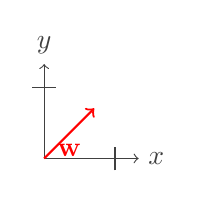
\begin{tikzpicture}[scale=.3]
    \draw [->,gray!50!black] (0,0)--(0,4) node[above]{$y$};
    \draw [->,gray!50!black] (0,0)--(4,0) node[right]{$x$};
    \draw [-,gray!50!black] (3,-0.5)--(3,0.5);
    \draw [-,gray!50!black] (-0.5,3)--(0.5,3);    

    \draw [->,red,thick] (0,0)--(2.12,2.12) node[midway,below] {$\mathbf{w}$};
    \end{tikzpicture}
    \end{center}
    
    \item Multiplying $\mathbf{v}$ by $\mathbf{A}$ rotated the vector counterclockwise by 45 degrees.
    
    \item First we compute
    $$\mathbf{u} = \mathbf{Bv} = \begin{bmatrix}
        \frac{\sqrt{3}}{2} \\ \frac{1}{2}
    \end{bmatrix}$$
    which is visually represented as
    \    \begin{center}
    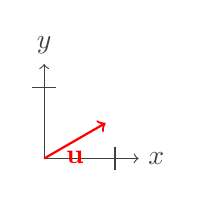
\begin{tikzpicture}[scale=.3]
    \draw [->,gray!50!black] (0,0)--(0,4) node[above]{$y$};
    \draw [->,gray!50!black] (0,0)--(4,0) node[right]{$x$};
    \draw [-,gray!50!black] (3,-0.5)--(3,0.5);
    \draw [-,gray!50!black] (-0.5,3)--(0.5,3);    

    \draw [->,red,thick] (0,0)--(2.6,1.5) node[midway,below] {$\mathbf{u}$};
    \end{tikzpicture}
    \end{center}
    
    \item Multiplying $\mathbf{v}$ by $\mathbf{B}$ rotated the vector counterclockwise by 30 degrees.
    
     \item First we compute
    $$\mathbf{t} = \mathbf{Rv} = \begin{bmatrix}
        \cos\theta \\ \sin\theta
    \end{bmatrix}$$
    which is visually represented as
    \begin{center}
    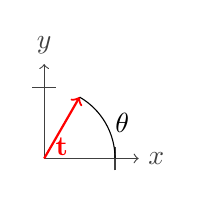
\begin{tikzpicture}[scale=.3]
    \draw [->,gray!50!black] (0,0)--(0,4) node[above]{$y$};
    \draw [->,gray!50!black] (0,0)--(4,0) node[right]{$x$};
    \draw [-,gray!50!black] (3,-0.5)--(3,0.5);
    \draw [-,gray!50!black] (-0.5,3)--(0.5,3);    

    \draw [->,red,thick] (0,0)--(1.5,2.6) node[midway,below] {$\mathbf{t}$};
    
    \draw (3,0) arc (0:60:3) node[right,midway]{$\theta$};
    \end{tikzpicture}
    \end{center}
    
    \item Multiplying $\mathbf{v}$ by $\mathbf{R}$ rotated the vector counterclockwise by $\theta$ degrees.
    
    \item The vector $\mathbf{w}$ is
    \begin{center}
    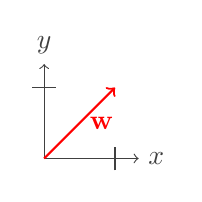
\begin{tikzpicture}[scale=.3]
    \draw [->,gray!50!black] (0,0)--(0,4) node[above]{$y$};
    \draw [->,gray!50!black] (0,0)--(4,0) node[right]{$x$};
    \draw [-,gray!50!black] (3,-0.5)--(3,0.5);
    \draw [-,gray!50!black] (-0.5,3)--(0.5,3);    

    \draw [->,red,thick] (0,0)--(3,3) node[midway,right] {$\mathbf{w}$};
        \end{tikzpicture}
    \end{center}
    
    \item First we compute
    $$\mathbf{s} = \mathbf{Rw} = \begin{bmatrix}
        \cos\theta - \sin\theta \\ \sin\theta + \cos\theta
    \end{bmatrix}$$
    which is visually represented
    \begin{center}
    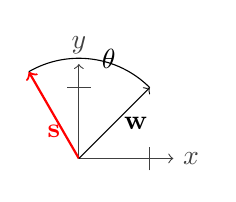
\begin{tikzpicture}[scale=.3]
    \draw [->,gray!50!black] (0,0)--(0,4) node[above]{$y$};
    \draw [->,gray!50!black] (0,0)--(4,0) node[right]{$x$};
    \draw [-,gray!50!black] (3,-0.5)--(3,0.5);
    \draw [-,gray!50!black] (-0.5,3)--(0.5,3);    

    \draw [->,red,thick] (0,0)--(-2.12,3.67) node[midway,below] {$\mathbf{s}$};
    \draw [->] (0,0)--(3,3) node[midway,right]{$\mathbf{w}$};
    
    \draw (3,3) arc (45:120:4.24) node[right,midway]{$\theta$};
    \end{tikzpicture}
    \end{center}
    
    \item Multiplying any vector by $\mathbf{R}$ rotates it by $\theta$.
    
\end{enumerate}
\end{sol}

\begin{center}
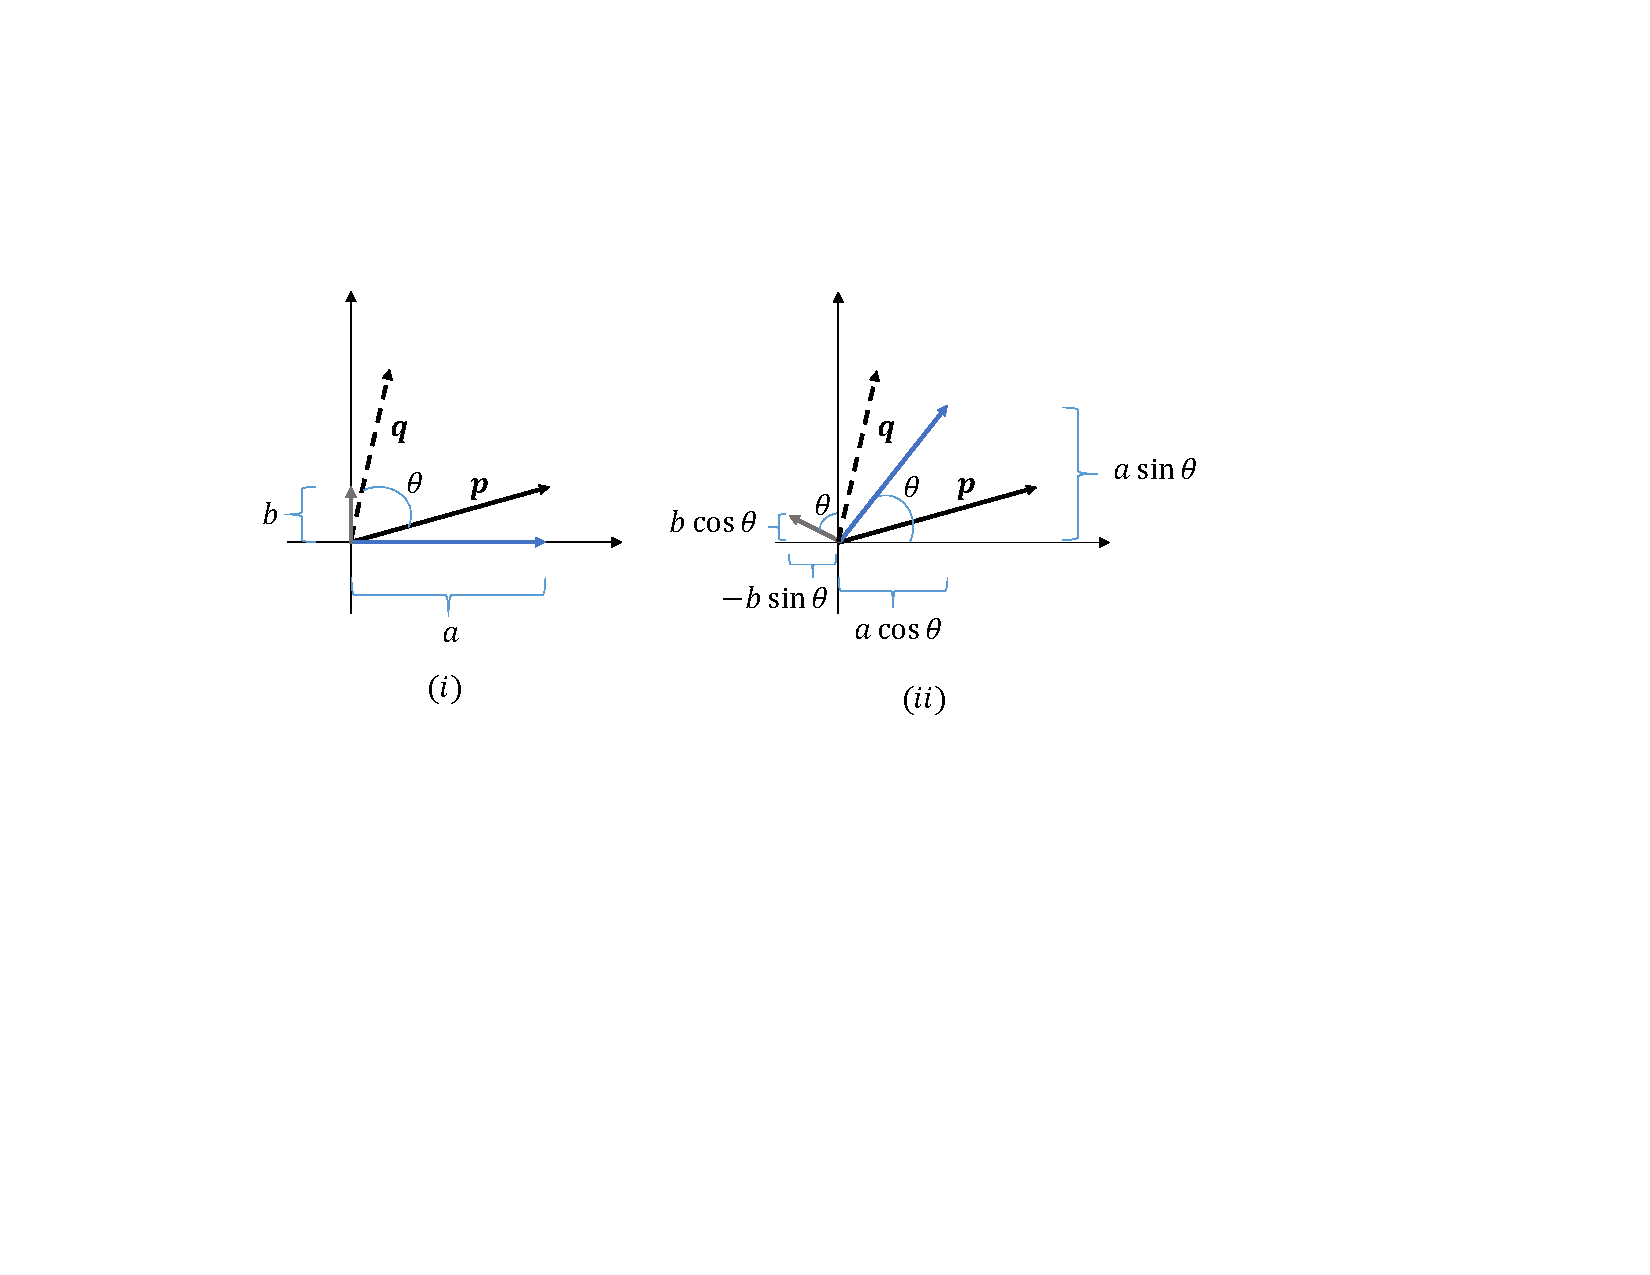
\includegraphics[width=4.5 in]{FacesDay1/figs/RotationMatrixDeriv.pdf}
\captionof{figure}{Rotation of vectors }
\label{fig:VecRotation}
\end{center}

You may have guessed that $\mathbf{R}$ defined above, rotates a vector counter-clockwise by $\theta$. This is indeed true, and $\mathbf{R}$ is called a \emph{rotation matrix} as it transforms vectors by rotating them. To understand why $\mathbf{R}$ is a rotation matrix, consider Figure \ref{fig:VecRotation} (i). Suppose that we wish to rotate the vector $\mathbf{p}$ counter-clockwise by $\theta$, which will result in the vector $\mathbf{q}$. From the figure, we see that
\begin{align}
\mathbf{p} =
\begin{bmatrix}
a \\ b
\end{bmatrix},
\end{align}
and $\mathbf{p}$ is the sum of the gray and blue vectors. If we now rotate the blue and gray vectors counter-clockwise by $\theta$, we see that $\mathbf{q}$ is the sum of the rotated versions of the blue and gray vectors, as shown in  Figure \ref{fig:VecRotation} (ii).  By using trigonometry, we see that the blue vector in  Figure \ref{fig:VecRotation} (ii) is
\begin{align}
\begin{pmatrix}
a\cos \theta\\
a \sin \theta
\end{pmatrix}
\end{align}
and the gray vector in  Figure \ref{fig:VecRotation} (ii) is
\begin{align}
\begin{pmatrix}
-b\sin \theta\\
b \cos \theta
\end{pmatrix}
\end{align}
Therefore, $\mathbf{q}$ is given by
\begin{align}
\mathbf{q}=
\begin{pmatrix}
a\cos \theta\\
a \sin \theta
\end{pmatrix}
+\begin{pmatrix}
-b\sin \theta\\
b \cos \theta
\end{pmatrix}=
+\begin{pmatrix}
a\cos \theta-b\sin \theta\\
a \sin \theta + b \cos \theta
\end{pmatrix} =\mathbf{Rp}.
\end{align}


\subsection{General Notation}
As we mentioned earlier, $m\times n$ matrices can multiply $n\times 1$ vectors and produce $m\times 1$ vectors. Consider  a generic $m \times n$ matrix $\mathbf{A}$
\begin{align*}
\mathbf{A} =
\begin{bmatrix}
    a_{11} & a_{12}& \cdots & a_{1n}\\
    a_{21} & a_{22} & \cdots & a_{2n}  \\
    \vdots & \cdots & \ddots & \vdots\\
    a_{m1} & a_{m2} & \cdots & a_{mn}
  \end{bmatrix}
\end{align*}
where the $ij$-th entry of this matrix, $a_{ij}$ defined above, is the entry corresponding to the $i$-th row and $j$-th column.
You can multiply an  $n\times 1$ vector $\mathbf{v}$ by this matrix. Define the vector $\mathbf{v}$ as follows,
\begin{align*}
\mathbf{v } =
\begin{bmatrix}
    v_{1}\\
    v_{2}\\
    \vdots\\
    v_{n}
  \end{bmatrix}.
\end{align*}
Now define another vector $\mathbf{w}$ which is the product of $\mathbf{A}$ and $\mathbf{v}$, i.e., $\mathbf{w} = \mathbf{Av}$. If we define
\begin{align*}
\mathbf{w} =
\begin{bmatrix}
    w_{1}\\
    w_{2}\\
    \vdots\\
    w_{m}
  \end{bmatrix}
\end{align*}
then the $i$-th entry of $\mathbf{w}$, is given by the following sum
\begin{align*}
w_{i} = a_{i1}v_{1} + a_{i2}v_2 \cdots a_{im}v_m = \sum_{j = 1}^n a_{ij}v_{j}
\end{align*}

\subsection{Other Matrix operations}
Besides multiplication, a number of other operations can be done using matrices including addition, subtraction, inversion, transposition, etc. We will explore more of these and their associated properties in the next section.  All of these operations make matrices a very powerful tool in the study of many different systems which can be represented as linear transformations, or combinations.

\section{Matrix Operations in MATLAB}
\begin{prob}
In the command window, you can type in commands and press enter. Try the following commands and see what they do.
\begin{lstlisting}
1+1
a=1+1
a
% you can start a comment with "%"
b=2;% this will appear as a variable in your workspace, but the semicolon suppresses the output
c=3,d=4,e=5;% use commas, semicolons, or shift+enter between commands that you want to execute together
1+2-(3*4/5)^6
clear a
a% should give you an error because a is not defined anymore
clear all
clc% only if you want to clear your workspace!
\end{lstlisting}
\end{prob}

To practice matrix operations, let's define a matrix and some vectors using MATLAB as follows:
\begin{lstlisting}
>> A = [2 1; 3 -1; 0 4]
\end{lstlisting}
Note that the semi-colon ends a row and begins a new row. You can also use returns between rows---try it! Square brackets enclose the matrix. To define the column vector $\mathbf{v}$ in MATLAB you can type the following command:
\begin{lstlisting}
>>  v = [-2; 1]
\end{lstlisting}
whilst to define the row vector $\mathbf{u}$ in MATLAB you can type the following command
\begin{lstlisting}
>>  u = [2 -3 1]
\end{lstlisting}
Notice that in this case each component of the vector is separated by a space - you could also separate them with a comma. 

\begin{prob}
Using the definitions for $\mathbf{A}$, $\mathbf{v}$, and $\mathbf{u}$ from above, please predict the output of the following commands and then solve them using MATLAB.

\begin{lstlisting}
A*v
u*A
A(1:2,:)*v
u*A(:,2)
\end{lstlisting}
\end{prob}

For Night 1, you will also need to plot things. In MATLAB, you can use plot(xv,yv) to create a scatter plot.
\begin{lstlisting}
yv=[1 7 4 5 3 9 2 4]
xv=[1 3 4 6 8 9 11 14]
plot(xv,yv)
\end{lstlisting}

If you want to know more about how to use a function like plot, use "help." Create the plot above, then type "help plot" into the command window and try to change something about your plot, such as using points instead of a line or adding axis labels.

Finally, you need to know how to use a for loop to repeat a set of commands a number of times. Here's an example for loop that makes a vector that's a sequence of squares: (Try it!)
\begin{lstlisting}
for n=1:3% n is the index variable, which counts from 1 to 3 (call it whatever you want)
v(n)=n^2% assigns the nth component of v to the value n^2 and prints out v
% loop repeats, adding 1 to n each time, until i gets to 3
end% needed to end the loop!
\end{lstlisting}

\begin{prob}
Write a for loop that creates the following matrix:
\begin{lstlisting}
M_squares=[1 1;2 4;3 9;4 16]
\end{lstlisting}
\end{prob}

\begin{sol}
\begin{lstlisting}
for n=1:4
M_squares(n,1) = n; %assigns the nth row, 1st column the value n
M_squares(n,2) = n^2; %assigns the nth row, 2nd column the value n^2
end
\end{lstlisting}
\end{sol}

\section{Elementary Matrix Operations, Properties, and Terminology}

In this part of the assignment, you will learn a number of basic operations and properties of matrices which can then be used in applications.  Admittedly, most of these exercises are a little dry, but they will be useful in the very near future, we promise!

\subsection{Matrix-Vector Multiply}

Here, you will work on examples of matrices multiplying vectors to get yourselves comfortable with matrix operations in MATLAB.  First, let's define the matrix $\A$ using MATLAB as follows

\begin{verbatim}
>> A = [2 1; 3 -1; 0 4]
\end{verbatim}
Note that the semi-colon ends a row and begins a new row. To define the column vector $\v$ in MATLAB you can type the following command:
\begin{verbatim}
>>  v = [-2; 1]
\end{verbatim}
whilst to define the row vector $\u$ in MATLAB you can type the following command
\begin{verbatim}
>>  u = [2 -3 1]
\end{verbatim}
Notice that in this case each component of the vector is separated by a space - you could also separate them with a comma.

\begin{prob}
Using the definitions for $\A$, $\v$, and $\mathbf{u}$ from above, please solve the following using MATLAB. Do the answers match what you expect? (Not all of these may be defined!)

\begin{enumerate}
    \item 
\begin{verbatim}
A*v
\end{verbatim}
\item
\begin{verbatim}
u*A
\end{verbatim}
\item 
\begin{verbatim}
A*u
\end{verbatim}
\item 
\begin{verbatim}
v*A
\end{verbatim}
\item 
\begin{verbatim}
A(1:2,:)*v
\end{verbatim}
\item 
\begin{verbatim}
u*A(:,2)
\end{verbatim}
\item 
\begin{verbatim}
A(:, 2:4)*v
\end{verbatim}
\item 
\begin{verbatim}
u*A(1,:)
\end{verbatim}
\end{enumerate}
\end{prob}

\begin{sol}
\begin{enumerate}
    \item \begin{verbatim}[-3; -7; 4]\end{verbatim}
    \item \begin{verbatim}[-5 9]\end{verbatim}
    \item Does not work because the inner matrix dimensions must agree and here we have a $3\times 2$ matrix multiplied by a $1\times 3$ matrix
    \item Does not work because the inner matrix dimensions must agree and here we have a $2\times 1$ matrix multiplied by a $3\times 2$ matrix
    \item \begin{verbatim}[-3; -7]\end{verbatim}
    \item 9
    \item Does not work because the index exceeds matrix dimensions. It is trying to access columns 2-4 of a two column matrix.
    \item Does not work because the inner matrix dimensions must agree and here we have a $1\times 3$ matrix multiplied by a $1\times 2$ matrix.
    \end{enumerate}
\end{sol}

\subsection{Addition, subtraction, scalar multiplication and transpose of matrices}

We can add matrices of the same size, and subtract them from one another. Both operations result in matrices of the same size and shape.  The addition and subtraction operations are done element-wise. For instance the difference of the two matrices can be calculated as below

\begin{align}
\mathbf{A} &= \begin{bmatrix}3 & 4 & 1 \\ 3 & 1 & 1 \end{bmatrix}\\
\mathbf{B} &= \begin{bmatrix}
1 & 2 & 3 \\ 2 & 2 & 1
\end{bmatrix}\\
\mathbf{A} - \mathbf{B} &= \begin{bmatrix}
(3 - 1) & (4-2) & (1-3) \\ (3-2) & (2-1) & (1-1)
\end{bmatrix} \\
&= \begin{bmatrix}
2 & 2 & -2 \\ 1 & -1 & 0
\end{bmatrix}
\end{align}

Multiplying a matrix by a scalar simply scales each entry of the matrix by the scale factor. For instance
\begin{align}
3 \mathbf{A} = \begin{bmatrix}
9 & 12 & 3\\
9 & 3 & 3
\end{bmatrix}
\end{align}

The transpose of a vector, denoted by the superscript $^T$ turns a column vector into a row vector, and vice versa. For matrices, the transpose replaces the rows with the columns (or vice-versa).  For example,

\begin{align}
\begin{bmatrix}
1 & 3 & 5 \\
2 & 7 & 6
\end{bmatrix}^T =
\begin{bmatrix}
1 & 2 \\
3 & 7 \\
5 & 6
\end{bmatrix}
\end{align}
Since the columns are replaced with the rows, the shape of the matrix changes when you transpose it.  The following property of transposes will be useful moving forward. Consider a matrix $\mathbf{A}$ and a vector $\mathbf{v}$. Then
\begin{align}
\left(\mathbf{Av}\right)^T = \mathbf{v}^T \mathbf{A}^T
\end{align}

\begin{prob}
Using $\mathbf{A}$ and $\mathbf{B}$ previously defined, evaluate $4\mathbf{A} - 5\mathbf{B}$
\end{prob}
\begin{sol}
\begin{align}4\mathbf{A} - 5\mathbf{B} =
\begin{bmatrix}
7 & 6 & -11\\
2 & -6 & -1
\end{bmatrix}
\end{align}
\end{sol}
\begin{prob}
If the matrix $\mathbf{A}$ has dimensions of $4\times 5$, what are the dimensions of $\mathbf{A}^T$?
\end{prob}
\begin{sol}
The dimensions of $\mathbf{A}^T$ are $5 \times 4$.
\end{sol}
\begin{prob}
If the matrix $\mathbf{A}$ is $4\times 5$ (i.e., $\mathbf{A}$ has dimensions $4 \times 5$) and the vector $\mathbf{v}$ is $5\times 1$, what are the dimensions of $\mathbf{Av}$ and $(\mathbf{Av})^T$?
\end{prob}
\begin{sol}
$\mathbf{Av}$ is $4 \times 1$ and $(\mathbf{Av})^T$ is $1 \times 4$.
\end{sol}
\begin{prob}
How do you find the transpose of a vector or matrix in MATLAB?
\end{prob}
\begin{sol}
You use the apostrophe: $(\mathbf{A})^T$ is \texttt{A'} in Matlab.
\end{sol}


\subsection{Matrix-Matrix Multiply}

Matrices can be multiplied together to produce other matrices. In general, when you multiply a matrix $\mathbf{A}$ with another matrix $\mathbf{B}$, you need the matrix on the left side of the product to have the same number of columns as the number of rows in the matrix on the right side. In other words if $\mathbf{A}$ is $m\times n$, and $\mathbf{B}$ is $p\times q$, you need $n = p$ for the product $\mathbf{C} = \mathbf{AB}$ to be defined. The product results in a new matrix $\mathbf{C}$ which is $m\times q$. The $q$ columns of the product matrix $\mathbf{C}$ are precisely the $q$ vectors that would result from multiplying $\mathbf{A}$ with the vectors formed by the columns of $\mathbf{B}$.

Consider the following matrices
\[ \mathbf{A} = \twobytwo{2}{1}{3}{-1} \hspace{1cm}
\mathbf{B} =
\left[\begin{array}{rr}
1 & 5 \\
-2 & 3
\end{array}\right].
\]
The product of the two $\mathbf{C} = \mathbf{AB}$ is computed as follows
\[ \mathbf{C} =
\left[\begin{array}{rr}
2 & 1 \\
3 & -1
\end{array}\right]
\left[\begin{array}{rr}
1 & 5 \\
-2 & 3
\end{array}\right]
=
\left[
\begin{array}{cc}
(2)(1) + (1)(-2) & (2)(5) + (1)(3) \\
(3)(1) + (-1)(-2)  & (3)(5)  + (-1)(3)
\end{array}
\right]
=
\left[
\begin{array}{rr}
0 & 13 \\
5 & 12
\end{array}
\right]
\]

As a second example consider the matrices $\mathbf{A}$ and $\mathbf{B}$ defined below, and let the product $\mathbf{C} = \mathbf{AB}$.

\[
\mathbf{A} =
\begin{bmatrix}
1 & 2 \\
3 & 2 \\
4 & 1
\end{bmatrix}
\mathbf{B} =
\begin{bmatrix}
1 & 4 \\
2 & 3
\end{bmatrix}
\]
\[
\mathbf{C} =
\begin{bmatrix}
(1)(1) + (2)(2) & (1)(4)+(2)(3) \\
(3)(1) + (2)(2) & (3)(4)+(2)(3) \\
(4)(1) + (1)(2) & (4)(4)+(1)(3)
\end{bmatrix}
 = \begin{bmatrix}
5 & 10 \\
7 & 18 \\
6 & 19
\end{bmatrix}
\]

As mentioned above, one way of envisioning matrix multiplication is if we consider the columns of input matrix $\mathbf{B}$ as a set of column vectors, we can multiply  these column vectors one at a time by the matrix $\mathbf{A}$, and the resulting vectors will be the corresponding columns of the output matrix $\mathbf{C}$, i.e.

\[\mathbf{A} \mathbf{B} = \mathbf{A} [\mathbf{B}_1, \mathbf{B}_2, \ldots] = [\mathbf{A} \mathbf{B}_1, \mathbf{A} \mathbf{B}_2, \ldots] \]
where $\mathbf{B}_1$ is the first column of matrix $\mathbf{B}$ etc.

Consider the following matrices:
\[ \mathbf{A} =
\left[\begin{array}{rr}
-2 & 4 \\
0 & 3
\end{array}\right]
\]
\[ \mathbf{B} =
\left[\begin{array}{rr}
5 & -3 \\
-1 & -1
\end{array}\right]
\]
\begin{prob}
Find the matrix product $\mathbf{A} \mathbf{B}$.
\end{prob}
\begin{sol}
\[ \mathbf{AB} =
\left[\begin{array}{rr}
-14 & 2 \\
-3 & -3
\end{array}\right]
\]
\end{sol}
\begin{prob}
Find the matrix product $\mathbf{B} \mathbf{A}$
\end{prob}
\begin{sol}
\[ \mathbf{BA} =
\left[\begin{array}{rr}
-10 & 11 \\
2 & -7
\end{array}\right]
\]
\end{sol}

Note that these two products are NOT equal.  In general, matrix multiplication, unlike scalar multiplication, is NOT commutative.  In other words, in general $\mathbf{A} \mathbf{B} \neq \mathbf{B} \mathbf{A}$.  However, the distributive property IS valid for matrices:  $\mathbf{A} (\mathbf{B} + \mathbf{C}) = \mathbf{A} \mathbf{B} + \mathbf{A} \mathbf{C}$ so long as we keep the order of the multiplication the same $(\mathbf{B} + \mathbf{C})\mathbf{A} = \mathbf{B} \mathbf{A} + \mathbf{C} \mathbf{A}$.  Recall the definition of matrix addition: if two matrices are of the same size then they can be added and each entry of the new matrix is the sum of the entries of the original matrices, e.g.
\[\left[\begin{array}{rr}
5 & -3 \\
-1 & -1
\end{array}\right] + \left[\begin{array}{rr}
4 & -2 \\
-3 & -1
\end{array}\right] = \left[\begin{array}{rr}
9 & -5 \\
-4 & -2
\end{array}\right]
\]

In addition to matrices $\mathbf{A}$ and $ \mathbf{B}$ defined above, consider the matrix
\[ \mathbf{C} =
\left[\begin{array}{rr}
-5 & -1 \\
-3 & 2
\end{array}\right]
\]

\begin{prob}
Calculate  $\mathbf{A} (\mathbf{B} + \mathbf{C}) $.
\end{prob}
\begin{sol}\[ \mathbf{A} (\mathbf{B} + \mathbf{C}) = \twobytwo{-16}{12}{-12}{3} \]
\end{sol}
\begin{prob}
Calculate  $\mathbf{A} \mathbf{B} + \mathbf{A} \mathbf{C}$. Is it equal to your previous answer?
\end{prob}
\begin{sol}It is the same answer, as expected, since you can distribute matrices.\end{sol}

Finally, since matrix multiplication is defined, there is no reason not to multiply a matrix by itself. This only works if it is a square matrix. (Think about why this is true.) Using $\mathbf{A}$ and $\mathbf{B}$ from above, evaluate the following expressions

\begin{prob}
\begin{enumerate}
\item $\mathbf{A}^2$
\item $\mathbf{B}^3$
\end{enumerate}
\end{prob}
\begin{sol}
\begin{enumerate}
    \item \[ \mathbf{A}^2 = \twobytwo{4}{4}{0}{9}\]
    \item $$B^3 = \begin{bmatrix}
    152 & -72 \\ -24 & 8
    \end{bmatrix}$$
\end{enumerate}
\end{sol}


\subsection{Special Types of Matrices}

\begin{prob}
There are lots of matrices that are special. Use a trusted linear algebra reference to define the following types of matrices, and provide an example of each:
\begin{enumerate}
\item Square Matrix
\item Rectangular Matrix
\item Diagonal Matrix
\item Identity Matrix
% \item Markov Matrix
\item Symmetric Matrix
% \item Skew-Symmetric Matrix
% \item Upper-Triangular Matrix
% \item Lower-Triangular Matrix
% \item Tridiagonal Matrix
\end{enumerate}
\end{prob}

\begin{sol}
\begin{enumerate}
    \item A square matrix is one that has size $n \times n$, e.g.,
\[ \left[ \begin{array}{rrr}
   * & * & * \\
   * & * & * \\
   * & * & *
 \end{array} \right].
\]

\item A rectangular matrix is one that has size $m \times n$ where $n$ is not equal to $m$, e.g.,

\[ \left[ \begin{array}{rrr}
   * & * & * \\
   * & * & * 
 \end{array} \right].
\]

\item A diagonal matrix is one whose only non-zero elements are on the diagonal from upper left to lower right, e.g.,

\[ \left[ \begin{array}{rrr}
   2 & 0 & 0 \\
   0 & 3 & 0 \\
   0 & 0 & 8
 \end{array} \right].
\]

\item The identity matrix is a square matrix with all zeroes except along the diagonal from the upper left to lower right, where the entries are all 1, e.g.,

\[ \left[ \begin{array}{rrr}
   1 & 0 & 0 \\
   0 & 1 & 0 \\
   0 & 0 & 1
 \end{array} \right].
\]

% \item An $n \times n$ matrix is called a Markov matrix if all entries are nonnegative and the sum of each column vector is equal to 1, e.g., for any $0\leq a,b\leq 1,$

% \[ \left[ \begin{array}{rr}
%   a & b \\
%   1-a & 1-b \\
%  \end{array} \right].
% \]

\item A matrix is symmetric if it is square and equal to its own transpose, i.e. $A=A^{T}$, e.g.,
\[ \left[ \begin{array}{rrr}
   1 & 7 & 3 \\
   7 & 4 & -5 \\
   3 & -5 & 6
 \end{array} \right].
\]

% \item A matrix is skew-symmetric if it is square and $-A=A^{T}$, e.g.,
% \[ \left[ \begin{array}{rrr}
%   0 & 2 & -1 \\
%   -2 & 0 & -4 \\
%   1 & 4 & 0
%  \end{array} \right].
% \]

% \item A square matrix is called upper triangular if all the entries below the main diagonal are zero, e.g.,
% \[ \left[ \begin{array}{rrr}
%   1 & 1 & 1 \\
%   0 & 1 & 1 \\
%   0 & 0 & 1
%  \end{array} \right].
% \]

% \item A square matrix is called lower triangular if all the entries above the main diagonal are zero, e.g., 
% \[ \left[ \begin{array}{rrr}
%   1 & 0 & 0 \\
%   1 & 1 & 0 \\
%   1 & 1 & 1
%  \end{array} \right].
% \]

% \item A tridiagonal matrix is a band matrix that has nonzero elements only on the main diagonal, the first diagonal below this, and the first diagonal above the main diagonal, e.g.,
% \[ \left[ \begin{array}{rrrrr}
%   1 & 1 & 0 & 0 & 0 \\
%   1 & 1 & 1 & 0 & 0  \\
%   0 & 1 & 1 & 1 & 0 \\
%  0 & 0 & 1 & 1 & 1 \\
%  0 & 0 & 0 & 1 & 1 \\
%  \end{array} \right]
% \]
\end{enumerate}
\end{sol}

\section{Matrices as transformation operators}

When matrices operate on (i.e., multiply) spatial position vectors, the vector which results is another spatial position vector.  The original spatial position has been 'transformed' into another position.  In particular, there are specific matrices which accomplish specific desired transformations. These are used in many different disciplines.

\subsection{Identity and Scaling Operations}
The matrix
\begin{equation}
\mathbf{I} = \left[ \begin{array}{ccc}
   1 & 0 & 0 \\
   0 & 1 & 0 \\
   0 & 0 & 1
 \end{array} \right]
\end{equation}
when multiplying the vector
\begin{align}
\mathbf{v} = \begin{bmatrix}
x\\y\\z
\end{bmatrix}
\end{align}
will reproduce the same vector, i.e. $\mathbf{I} \mathbf{v} = \mathbf{v}$.  For this reason, the matrix $\mathbf{I}$ above is called an identity matrix. Identity matrices in higher dimensions are defined the same way, i.e., a 4-dimensional identity matrix is a $4\times 4$ matrix with 1s on the diagonal and zeros everywhere else, i.e.,
\begin{equation}
 \left[ \begin{array}{cccc}
   1 & 0 & 0 & 0 \\
   0 & 1 & 0 & 0\\
   0 & 0 & 1 & 0 \\
   0 & 0 & 0 & 1 \\
 \end{array} \right]
\end{equation}

\begin{prob}
\begin{enumerate}
\item Another important and simple operation is to be able to take a vector and scale (increase or decrease its length) it by an overall multiplicative factor while maintaining its direction. Consider the vector

    \begin{align*}
    \mathbf{v} = \begin{bmatrix}
    x\\y\\z
    \end{bmatrix}
    \end{align*}
    Thinking about how the identity matrix acts on this vector, propose a $3\times 3$ matrix which scales this vector by a factor of $3$ to the vector
    \begin{align*}
    3\mathbf{v} = \begin{bmatrix}
    3x\\3y\\3z
    \end{bmatrix}.
    \end{align*}
    In other words, find a $3 \times 3$ matrix $\mathbf{M}$ such that $\mathbf{Mv} = 3\mathbf{v}$ for any vector $\mathbf{v}$.
\item  What if you want to scale the $x$ component differently than the $y$ component?  Write down the $3\times 3$ matrix which scales the $x$ component by $3$ and the $y$ component by $5$ and leaves the $z$ component the same.
\item Write down the $3 \times 3$ matrix which scales the $x$ component by $a$, the $y$ component by $b$, and the $z$ component by $c$.
\end{enumerate}
\end{prob}

\begin{sol}
\begin{enumerate}
    \item \[ \mathbf{M} = \left[\begin{array}{rrr} 3 & 0 & 0 \\ 0 & 3 & 0 \\ 0 & 0 & 3 \end{array}\right] \]
    \item \[ \mathbf{M} = \left[\begin{array}{rrr} 3 & 0 & 0 \\ 0 & 5 & 0 \\ 0 & 0 & 1 \end{array}\right] \]
    \item We can generalize the result: \[ \mathbf{M} = \left[\begin{array}{rrr} a & 0 & 0 \\ 0 & b & 0 \\ 0 & 0 & c \end{array}\right] \]
\end{enumerate}
\end{sol}

% JBG: I am going to comment out this next section since we need to shorten the assignment and we don't really need 3D operations just yet, and it would be better to introduce it during the day assignment anyway.

% \subsection{Rotation Operations in 3D}


% In class, you saw rotation matrices in  two dimensions. Here, we will extend those ideas to 3-dimensional vectors. First, let's start by building some intuition for what rotation matrices in 3D do.

% \begin{prob}
% \begin{enumerate}
%     \item Multiply the vectors
%     \begin{align}
%     \begin{bmatrix}
%     1\\0\\0\\
%     \end{bmatrix},\begin{bmatrix}
%     0\\1\\0\\
%     \end{bmatrix},\begin{bmatrix}
%     0\\0\\1\\
%     \end{bmatrix}
%     \end{align}
%      by the following matrix:
%     \begin{equation}
%     \mathbf{A} = \left[ \begin{array}{rrr}
%       0 & -1 & 0 \\
%       1 & 0 & 0 \\
%       0 & 0 & 1
%     \end{array} \right].
%     \end{equation}
%     What transformation does this matrix represent? (In other words, can you capture, in a single concept, what this matrix does to any vector?  Hint:  look at the section heading).
%     \item Similarly, consider multiplying the vectors
%     \begin{align}
%     \begin{bmatrix}
%     1\\0\\0\\
%     \end{bmatrix},\begin{bmatrix}
%     0\\1\\0\\
%     \end{bmatrix},\begin{bmatrix}
%     0\\0\\1\\
%     \end{bmatrix}
%     \end{align}
%     by the following matrix:
%     \begin{equation}
%     \mathbf{A} = \left[ \begin{array}{rrr}
%       1 & 0 & 0 \\
%       0 & 0 & -1 \\
%       0 & 1 & 0
%      \end{array} \right]
%     \end{equation}
%     What transformation does this matrix represent?

%     \item Lastly, what transformation does this matrix represent?
%     \begin{equation}
%     \mathbf{A} = \left[ \begin{array}{rrr}
%     0 & 0 & 1 \\
%   0 & 1 & 0 \\
%   -1 & 0 & 0
%      \end{array} \right]
%     \end{equation}
% \end{enumerate}
% \end{prob}
    

% \begin{sol}
% \begin{enumerate}
%     \item 
%     $$\mathbf{A}\begin{bmatrix} 1 \\ 0 \\ 0 \end{bmatrix} = \begin{bmatrix} 0 \\ -1 \\ 0 \end{bmatrix}$$ \\
%     $$\mathbf{A}\begin{bmatrix} 0 \\ 1 \\ 0 \end{bmatrix} = \begin{bmatrix} 1 \\ 0 \\ 0 \end{bmatrix}$$ \\
%     $$\mathbf{A}\begin{bmatrix} 0 \\ 0 \\ 1 \end{bmatrix} = \begin{bmatrix} 0 \\ 0 \\ 1 \end{bmatrix}$$

% This matrix is performing a $90^o$ counterclockwise rotation about the $z$-axis.  In order to see this, we recommend actually drawing these vectors in 3D. Can you see that the vector (1,0,0) (i.e., the x-axis) is rotated 90 degrees counterclockwise to align with the y-axis (0,1,0)? The y-axis (0,1,0) is rotated 90 degrees counterclockwise to align with the negative x-axis (-1,0,0). Finally, the z-axis (0,0,1) is left unchanged. The term we use to describe vectors which are offset by 90 degrees can vary, but you will most typically hear them referred to as \textbf{orthogonal} or \textbf{normal}.


% \item \begin{align*}
%     \mathbf{A}\begin{bmatrix} 1 \\ 0 \\ 0 \end{bmatrix} &= \begin{bmatrix} 1 \\ 0 \\ 0 \end{bmatrix} \\
%     \mathbf{A}\begin{bmatrix} 0 \\ 1 \\ 0 \end{bmatrix} &= \begin{bmatrix} 0 \\ 0 \\ -1 \end{bmatrix} \\
%     \mathbf{A}\begin{bmatrix} 0 \\ 0 \\ 1 \end{bmatrix} &= \begin{bmatrix} 0 \\ 1 \\ 0 \end{bmatrix}
% \end{align*}
% This matrix is performing a $90^o$ counterclockwise rotation about the $x$-axis: the x-axis (1,0,0) remains unchanged; the y-axis (0,1,0) becomes the z-axis (0,0,1); and the z-axis (0,0,1) becomes the negative y-axis (0,-1,0). 

% \item Let's take a closer look at what this matrix does:
% \begin{align*}
%     \mathbf{A}\begin{bmatrix} 1 \\ 0 \\ 0 \end{bmatrix} &= \begin{bmatrix} 0 \\ 0 \\ 1 \end{bmatrix} \\
%     \mathbf{A}\begin{bmatrix} 0 \\ 1 \\ 0 \end{bmatrix} &= \begin{bmatrix} 0 \\ 1 \\ 0 \end{bmatrix} \\
%     \mathbf{A}\begin{bmatrix} 0 \\ 0 \\ 1 \end{bmatrix} &= \begin{bmatrix} -1 \\ 0 \\ 0 \end{bmatrix}
% \end{align*}
% This matrix is performing a $90^o$ counterclockwise rotation about the $y$-axis: the y-axis (0,1,0) remains unchanged; the x-axis (1,0,0) becomes the negative z-axis (0,0,-1); and the z-axis (0,0,1) becomes the x-axis (1,0,0).
% \end{enumerate}
% \end{sol}


% So, hopefully by this point you have convinced yourself that the above matrices transform vectors by rotating them counterclockwise through an angle of 90 degrees about some coordinate axis.   What if we want to rotate the vector counterclockwise through an angle which is not 90 degrees? Consider the following matrix:

% \begin{equation}
% \mathbf{R} =  \left[ \begin{array}{rrr}
%   \cos \theta & -\sin \theta & 0  \\
%   \sin\theta & \cos \theta & 0  \\
%   0  & 0  &  1
%  \end{array} \right]
% \end{equation}


% \begin{prob}
%  What is this matrix equal to for $\theta = 0$?  What is it equal to for $\theta = 90$ degrees?
%  \end{prob}
%  \begin{sol}
% \begin{align*}
%     \mathbf{R} &= \mathbf{R}(\theta) \\
%     \mathbf{R}(0) &= \begin{bmatrix} 1 & 0 & 0 \\ 0 & 1 & 0 \\ 0  & 0  & 1 \end{bmatrix} \\
%     \mathbf{R}(90^o) &= \begin{bmatrix} 0 & -1 & 0 \\ 1 & 0 & 0 \\ 0  & 0  & 1 \end{bmatrix}
% \end{align*}

% For $\theta=0$, \textbf{R} simply becomes the identity matrix and no rotation is performed. For $\theta=90^o$, \textbf{R} becomes the $90^o$ counter-clockwise rotation about the $z$-axis we saw earlier.
% \end{sol}

% \begin{prob}
% If $\theta = \pi/2$ what is the result of multiplying this matrix and the vector $(1,0,0)$?
% \end{prob}
% \begin{sol}
% \begin{align*}
%     \mathbf{R}(\pi/2)\begin{bmatrix} 1 \\ 0 \\ 0 \end{bmatrix} &= \begin{bmatrix} 0 & -1 & 0 \\ 1 & 0 & 0 \\ 0  & 0  & 1 \end{bmatrix}\begin{bmatrix} 1 \\ 0 \\ 0 \end{bmatrix} \\
%     &= \begin{bmatrix} 0 \\ -1 \\ 0 \end{bmatrix}
% \end{align*}

% It's the same as a $90^o$ counter-clockwise rotation about the $z$ axis.\end{sol}

% \begin{prob}
% Let $$\mathbf{v} = \begin{bmatrix}
% a \\ b \\ c
% \end{bmatrix}$$ be a vector in 3D. Show that when we multiply $\mathbf{R}$ (for any value of $\theta$) by $\mathbf{v}$, the length (norm) of the vector is unchanged.   (Hint:  remember that $\cos^2\theta + \sin^2\theta = 1$).
% \end{prob}
% \begin{sol}
% \begin{align*}
%     \mathbf{u} &= \mathbf{Ru} \\ &= \mathbf{R}(\theta)\begin{bmatrix} a \\ b \\ c \end{bmatrix} \\
%     &= \begin{bmatrix} \cos\theta & -\sin\theta & 0 \\ \sin\theta & \cos\theta & 0 \\ 0  & 0  & 1 \end{bmatrix}\begin{bmatrix} a \\ b \\ c \end{bmatrix} \\
%     &= \begin{bmatrix} a\cos\theta - b\sin\theta \\ a\sin\theta + b\cos\theta \\ c \end{bmatrix} \\
% 	||{\mathbf{u}}|| &= \sqrt{\left(a\cos\theta - b\sin\theta\right)^2 + \left(a\sin\theta + b\cos\theta\right)^2 + c^2} \\
%     &= \sqrt{a^2\cos^2\theta - 2ab\cos\theta\sin\theta + b^2\sin^2\theta + a^2\sin^2\theta + 2ab\sin\theta\cos\theta + b^2\cos^2\theta + c^2} \\
%     &= \sqrt{a^2 + b^2 + c^2}
%     &= \|\mathbf{v}\|.
% \end{align*}
% \end{sol}

% \begin{prob}
% What transformation does this matrix represent?  By analogy, construct the rotation matrices for counterclockwise rotation by an angle $\theta$ around the other two coordinate axes. See the Wikipedia pages on "Rotation Matrix" for more information.
% \end{prob}
% \begin{sol}
% \begin{align*}
%     \mathbf{R}_{x} &= \begin{bmatrix} 1 & 0 & 0 \\ 0 & \cos\theta & -\sin\theta \\ 0 & \sin\theta & \cos\theta \end{bmatrix} \\
%     \mathbf{R}_{y} &= \begin{bmatrix} \cos\theta & 0 & \sin\theta \\ 0 & 1 & 0 \\ -\sin\theta  & 0 & \sin\theta \end{bmatrix} \\
%     \mathbf{R}_{z} &= \begin{bmatrix} \cos\theta & -\sin\theta & 0 \\ \sin\theta & \cos\theta & 0 \\ 0 & 0  & 1 \end{bmatrix}
% \end{align*}
% \end{sol}



%Now let's consider these principles using the transformation matrices we worked with above.
%
%
%\begin{enumerate}[resume]
%\item  Hold a closed book in front of you, with the top of the book towards the ceiling ($+z = (0,0,1)$ direction) and the front of the book pointed towards you ($+x = (1,0,0)$ direction), which leaves the opening side of the book pointing towards your right ($+y = (0,1,0)$).
%    \begin{enumerate}
%    \item  Rotate the book by 90 degrees clockwise about the $+x$ axis, then from this position, rotate the book by 90 degrees clockwise about the $+z$ axis.  Which direction is the cover of the book facing now?
%    \item  Return to the starting position.  Now rotate the book by 90 degrees clockwise about the $+z$ axis, and then from this position, rotate the book by 90 degrees clockwise about the $+x$ axis.  Which direction is the cover of the book facing now?  Is it the same as in part a?
%    \item  The cover of the book is originally pointed towards $(1,0,0)$.  Multiply this vector with the appropriate sequence of rotation matrices from above to reproduce your motions from part a.  Do you end up with the correct final cover direction?
%    \item  Multiply the $(1,0,0)$ vector with the appropriate sequence of rotation matrices to reproduce the motions from part b.  Do you end up with the correct final cover direction?
%    \item  From either of your answers to part c or part d, try, instead of operating on the $(1,0,0)$ vector sequentially with one rotation matrix and then the other, take the product of the two rotation matrices first, and then multiply $(1,0,0)$ with the resultant matrix.  Does this reproduce your answer?  What if you take the product the other way?
%    \end{enumerate}
%\item  If we want to rotate a vector $\mathbf{v}$ by an angle $\theta$ about the $z$ axis to get a vector $\mathbf{w}$, which matrix $\mathbf{R}$ do we use? Oops, now we changed our mind and decided we didn't want to do that after all.  What matrix $\mathbf{S}$ can we multiply $\mathbf{w}$ by to get back to $\mathbf{v}$?  $\mathbf{R}$ and $\mathbf{S}$ are known as inverses of each other.  What happens if we multiple these two matrices together?
%
%\end{enumerate}

\section{Data in Matrices and Vectors}

Most of the examples you saw up to now in this assignment involved vectors which represent spatial positions, and most of the matrices you encountered represent transformations of the spatial vectors. But, as you saw with the example involving fruits, vectors can also be used to store data. So can matrices.

For instance, you may have the following matrix

\begin{align}
\begin{bmatrix}
41 & 35 & 37 & 43 \\
49 & 40 & 48 & 61
\end{bmatrix}
\end{align}
whose first row represents the forecasted high temperature in Needham for the next 4 days (as of the day this was written) and the second row represents the forecasted high temperatures for Washington DC. By representing this data in matrix form, you can do a number of operations to help extract useful information from the data.

\begin{prob}
For this exercise, you will work with historical temperature data for the cities of Boston, Providence, Washington DC and New York.
\begin{enumerate}
\item Download the file \texttt{temps.mat} from canvas and load the data in it into MATLAB using \texttt{>> load temps.mat}. You should now have access to a matrix \texttt{T} which contains daily average temperatures from 1995 to 2015 for the cities of Boston, Providence, Washington DC and New York (we are not telling you in what order yet). By using MATLAB's \texttt{size} function, determine the dimensions of this matrix. Are the temperatures for each city contained in the rows or the columns of this matrix?
\item The data provided is given in Fahrenheit, and suppose you wish to convert it to Celsius using matrix operations (note that there are a number of ways of doing this, but we are focusing on using matrices here). The formula for converting a Fahrenheit temperature to Celsius is to first subtract 32 from the Fahrenheit temperature, and multiply the result by $\frac59$.

    \begin{enumerate}
    \item Define a matrix of the same shape as \texttt{T} with all its entries equalling 32, and call this matrix \texttt{B}. You will find MATLAB's \texttt{ones} function, which generates a matrix filled with 1's, useful here.
    
    \item Define a square, diagonal matrix of the appropriate dimensions which when multiplying another matrix scales all its entries by $\frac59$.  You should call this matrix \texttt{A}. You will find MATLAB's \texttt{eye} function, which generates an identity matrix, useful here.
    
    \item Using your answers to the previous parts and appropriate matrix operations, please provide 1 line of MATLAB code which generates a new matrix \texttt{Y} which contains the temperature data in Celsius.
    \end{enumerate}

\item Lets go back to Fahrenheit for the rest of the assignment. Extract the temperatures for each city into 4 different vectors \texttt{t1, t2, t3, t4}, and check that the dimensions of these vectors are as expected.

\item Using MATLAB's mean function, which computes the average of the values in a vector, and guess, based on geography, which of the vectors corresponds to the temperature for which city.

\item What are the maximum and minimum temperatures for Boston in the 20 years for which you have data?

\item On the same axes, plot graphs for the daily temperatures for the four cities for the last year for which you have data. Use MATLAB's \texttt{legend, xlabel, ylabel} functions to label the graphs.

\item Suppose that a genie told you that you can guess the temperature of New York, which we call $T_n$, using the temperatures of Boston, Providence, and Washington DC, which we respectively call $T_b$, $T_p$ and $T_w$. From the matrix \texttt{T}, extract a $3 \times 365$ matrix of daily temperatures for the last year (for which you have data) in Boston, Providence and Washington DC.

\item The genie says that a good approximation for the temperature on a given day in New York is given by
    \begin{align}
    T_n \approx 0.2235 T_b + 0.4193 T_p + 0.3856 T_w.
    \end{align}
    Formulate a matrix equation which uses the matrix from the previous part and the formula from the genie to guess the daily temperature in New York for the last year. Apply this equation in MATLAB.
    
    \item On the same axes, plot your prediction for the temperature in New York from the previous part, and the true temperature data which you extract from \texttt{T}. Is the prediction close?
\end{enumerate}

In the course of this module, you will learn how to come up with the coefficients we provided here using historical data. (No, we don't actually have a genie.)
\end{prob}

\begin{sol}
\begin{enumerate}
    \item After loading the temperatures you can see that they are stored inside a matrix called T which has 4 rows and 7670 columns, so presumably the temperature for each city is stored in a row.
    \item
        \begin{enumerate}
            \item We can define a matrix B of the same size as T but filled with 1s by typing \texttt{>> B = ones(4,7670)} and then we can multiply it by 32 by typing \texttt{>> B = 32*B}. Alternatively we could include the 32 from the start by typing \texttt{>> B = 32*ones(4,7670)}
            \item There are two ways to do this: we can multiply either on the left or right.
            \begin{itemize}
                \item Option 1: To multiply a $4\times 7670$ matrix on the left, we need a $4 \times 4$ matrix, which we would create by typing \texttt{>>  A = eyes(4)*5/9}.
                \item Option 2: To multiply a $4\times 7670$ matrix on the left, we need a $7670 \times 7670$ matrix, which we would create by typing \texttt{>>  A = eyes(7670)*5/9}.
            \end{itemize}
            \item Now that we have the pieces in place we could simply type \texttt{>> Y = A*(T-B)} (or \texttt{Y = (T-B)*A} if you chose the right multiply option). We can actually make this a lot simpler because MATLAB will create matrices of the correct size on the fly, so the following will work \texttt{>> Y = (T-32)*5/9}. Normally we would expect \texttt{T-32} to be a problem because we are subtracting a scalar from a matrix, but MATLAB simply assumes that we wish to subtract 32 from every element in the matrix.
        \end{enumerate}
        
        \item We can extract the first temperature by typing the following \texttt{>> t1 = T(1,:)} - this simply grabs all of the elements in the first row, so that \texttt{t1} should be a row vector of size 1 by 7670. We create the other vectors in a similar way.
        
        \item We can take the mean of the first city by typing \texttt{>> mean(t1)} and we get 51.7667. The other means respectively are 51.9140, 58.4365, and 55.9451. A little bit of geography suggests that the cities are ordered as follows: Boston, Providence, DC, New York.
        
        \item We can compute the maximum by typing \texttt{>> max(t1)} and we get 90.7. The minimum is 0.7.
        
        \item We are only supposed to grab the last year (365 days) so for Boston we would type \texttt{>> plot(t1(end-364:end))}, or we could use the actual size of the vector.
        
        \item Boston, Providence, and DC are stored in the first three rows. We'll extract their data and store it in a new matrix S by typing \texttt{>> S = T(1:3,end-364:end)}, which grabs the first three rows and the last 365 entries.
        
        \item We can define Tn by typing \texttt{>> Tn = 0.2235*S(1,:) + 0.4193*S(2,:) + 0.3856*S(3,:)} since the city temperatures are stored in the each of the three rows of the matrix S.
        
        \item Graphically they look pretty good. We can also examine the data a little more closely by looking at the difference between the predicted temperature and the actual temperature - it fluctuates with a mean of roughly 8.8115e-04, a maximum of 7.5334, and a minimum of -6.8966. Compared to the actual temperatures this implies that the prediction is never any worse than roughly 10\%.
\end{enumerate}
\end{sol}

\section{Conceptual Quiz}
Please figure out the answer to these questions and mark your answer in Canvas. You can retake the quiz, as needed.

\begin{enumerate}
\item $\mathbf{A}$ is a $3 \times 4$ matrix and $\mathbf{B}$ is a $4\times 2$ matrix. What is the size of $\mathbf{A} \mathbf{B}$?
\begin{tabbing}
  Column 1 \= Column 2 \kill
  % \> for next tab, \\ for new line...
  A. $ 2 \times 3$   \\
  B. $3\times 1$ \\
  C. $3 \times 2$ \\
  D.  The product is not defined.
\end{tabbing}
\item What is the result of the following matrix product
\begin{align*}
\begin{bmatrix}
1 & 2 & -3 \\
2 & -2 & 4 \\ 3 & -4 & 5
\end{bmatrix}
\begin{bmatrix}
 4 & 2 \\-3 & -3 \\ 1  & 1
\end{bmatrix}
\end{align*}

  A. \vspace{-2em}\begin{align*}
  \begin{bmatrix}
   -5 &   -7 \\
    18  &  14 \\
    24  &  23
    \end{bmatrix}
    \end{align*}

  B. \vspace{-2em}\begin{align*}
  \begin{bmatrix}
   -5 &   -7 \\
    18  &  14 \\
    29  &  23
    \end{bmatrix}
    \end{align*}
  C.\vspace{-2em} \begin{align*}
  \begin{bmatrix}
   -5 &  18 & 24 \\
   -7 & 14 & 23
    \end{bmatrix}
    \end{align*}

  D.\vspace{-2em} \begin{align*}
  \threebythree{-5}{-7}{3}{18}{14}{6}{24}{23}{9}
  \end{align*}

\item Match the following items (* means any number):

\begin{tabular}{ll}
1. Rectangular Matrix & A. $\threebythree{1}{0}{0}{0}{1}{0}{0}{0}{1}$ \\
2. Diagonal Matrix & B. $\threebythree{1}{2}{3}{2}{4}{5}{3}{5}{6}$ \\
3. Identity Matrix & C. $\threebythree{*}{0}{0}{0}{*}{0}{0}{0}{*}$ \\
4. Symmetric Matrix & D. $\threebytwo{*}{*}{*}{*}{*}{*}$
\end{tabular}

\item Which of the following matrices will scale the length of any 2-D vector by $\frac12$ ?

A. \begin{align*}
\begin{bmatrix} \frac12 & 0 \\ 0 & \frac12 \end{bmatrix}
    \end{align*}

B. \begin{align*}
\begin{bmatrix} \frac{1}{\sqrt{2}} & 0 \\ 0 & \frac{1}{\sqrt{2}}  \end{bmatrix}
    \end{align*}

C. \begin{align*}
\begin{bmatrix} \frac{1}{2} & 0 \\ 0 &  1 \end{bmatrix}
    \end{align*}

D. \begin{align*}
\begin{bmatrix}\frac{1}{2} & \frac12 \\ \frac12 & \frac12\end{bmatrix}
    \end{align*}

\item All of the following vectors are unit length. In which picture is $\mathbf{v}\cdot\mathbf{w}$ the largest?

A.     \begin{center}
    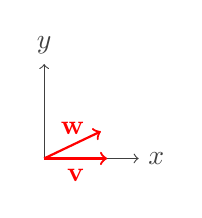
\begin{tikzpicture}[scale=0.8]
    \draw [->,gray!50!black] (0,0)--(0,1.5) node[above]{$y$};
    \draw [->,gray!50!black] (0,0)--(1.5,0) node[right]{$x$};  

    \draw [->,red,thick] (0,0)--(1,0) node[midway,below] {$\mathbf{v}$};
    \draw [->,red,thick] (0,0)--(.9,.43) node[midway,above] {$\mathbf{w}$};
        \end{tikzpicture}
    \end{center}
    
B. \begin{center}
    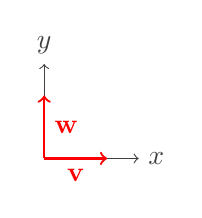
\begin{tikzpicture}[scale=0.8]
    \draw [->,gray!50!black] (0,0)--(0,1.5) node[above]{$y$};
    \draw [->,gray!50!black] (0,0)--(1.5,0) node[right]{$x$};  

    \draw [->,red,thick] (0,0)--(1,0) node[midway,below] {$\mathbf{v}$};
    \draw [->,red,thick] (0,0)--(0,1) node[midway,right] {$\mathbf{w}$};
        \end{tikzpicture}
    \end{center}
    
C. \begin{center}
    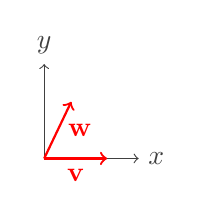
\begin{tikzpicture}[scale=0.8]
    \draw [->,gray!50!black] (0,0)--(0,1.5) node[above]{$y$};
    \draw [->,gray!50!black] (0,0)--(1.5,0) node[right]{$x$};  

    \draw [->,red,thick] (0,0)--(1,0) node[midway,below] {$\mathbf{v}$};
    \draw [->,red,thick] (0,0)--(.43,.9) node[midway,right] {$\mathbf{w}$};
        \end{tikzpicture}
    \end{center}
    
D. \begin{center}
    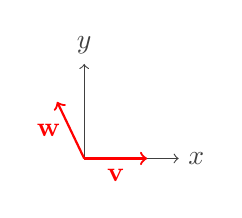
\begin{tikzpicture}[scale=0.8]
    \draw [->,gray!50!black] (0,0)--(0,1.5) node[above]{$y$};
    \draw [->,gray!50!black] (0,0)--(1.5,0) node[right]{$x$};  

    \draw [->,red,thick] (0,0)--(1,0) node[midway,below] {$\mathbf{v}$};
    \draw [->,red,thick] (0,0)--(-.43,.9) node[midway,left] {$\mathbf{w}$};
        \end{tikzpicture}
    \end{center}

\end{enumerate}

\pagebreak

\shipoutAnswer
